% !TEX TS-program = XeLaTeX
% use the following command:
% all document files must be coded in UTF-8
\documentclass[english]{textolivre}
% build HTML with: make4ht -e build.lua -c textolivre.cfg -x -u article "fn-in,svg,pic-align"

\journalname{Texto Livre}
\thevolume{16}
%\thenumber{1} % old template
\theyear{2023}
\receiveddate{\DTMdisplaydate{2022}{11}{15}{-1}} % YYYY MM DD
\accepteddate{\DTMdisplaydate{2022}{11}{29}{-1}}
\publisheddate{\DTMdisplaydate{2023}{1}{6}{-1}}
\corrauthor{Ester Trigo Ibanez}
\articledoi{10.1590/1983-3652.2023.41798}
%\articleid{NNNN} % if the article ID is not the last 5 numbers of its DOI, provide it using \articleid{} commmand 
% list of available sesscions in the journal: articles, dossier, reports, essays, reviews, interviews, editorial
\articlesessionname{dossier}
\runningauthor{Trigo Ibanez and Santos Díaz} 
%\editorname{Leonardo Araújo} % old template
\sectioneditorname{Hugo Heredia Ponce}
\layouteditorname{Daniervelin Pereira}

\title{Virtual tools in the concept of reading of future teachers: a lexical exploration}
\othertitle{Ferramentas virtuais na concepção de leitura de futuros professores: uma exploração lexical}
% if there is a third language title, add here:
%\othertitle{Artikelvorlage zur Einreichung beim Texto Livre Journal}

\author[1]{Ester Trigo Ibanez~\orcid{0000-0003-3035-4398}\thanks{Email: \href{mailto:ester.trigo@uca.es}{ester.trigo@uca.es}}}
\author[2]{Inmaculada Clotilde Santos Díaz~\orcid{0000-0002-0066-7783}\thanks{Email: \href{mailto:santosdiaz@uma.es}{santosdiaz@uma.es}}}
\affil[1]{Facultad de Ciencias de la educación, Departamento de Didáctica de la Lengua y la Literatura, Cádiz, España.}
\affil[2]{Universidad de Málaga, Facultad de Ciencias de la Educación, Departamento de Didáctica de las lenguas, las artes y el deporte, Málaga, España.}

\addbibresource{article.bib}
% use biber instead of bibtex
% $ biber article

% used to create dummy text for the template file
\definecolor{dark-gray}{gray}{0.35} % color used to display dummy texts
\usepackage{lipsum}
\SetLipsumParListSurrounders{\colorlet{oldcolor}{.}\color{dark-gray}}{\color{oldcolor}}

% used here only to provide the XeLaTeX and BibTeX logos
\usepackage{hologo}

% if you use multirows in a table, include the multirow package
\usepackage{multirow}

% provides sidewaysfigure environment
\usepackage{rotating}

% CUSTOM EPIGRAPH - BEGIN 
%%% https://tex.stackexchange.com/questions/193178/specific-epigraph-style
\usepackage{epigraph}
\renewcommand\textflush{flushright}
\makeatletter
\newlength\epitextskip
\pretocmd{\@epitext}{\em}{}{}
\apptocmd{\@epitext}{\em}{}{}
\patchcmd{\epigraph}{\@epitext{#1}\\}{\@epitext{#1}\\[\epitextskip]}{}{}
\makeatother
\setlength\epigraphrule{0pt}
\setlength\epitextskip{0.5ex}
\setlength\epigraphwidth{.7\textwidth}
% CUSTOM EPIGRAPH - END

% LANGUAGE - BEGIN
% ARABIC
% for languages that use special fonts, you must provide the typeface that will be used
% \setotherlanguage{arabic}
% \newfontfamily\arabicfont[Script=Arabic]{Amiri}
% \newfontfamily\arabicfontsf[Script=Arabic]{Amiri}
% \newfontfamily\arabicfonttt[Script=Arabic]{Amiri}
%
% in the article, to add arabic text use: \textlang{arabic}{ ... }
%
% RUSSIAN
% for russian text we also need to define fonts with support for Cyrillic script
% \usepackage{fontspec}
% \setotherlanguage{russian}
% \newfontfamily\cyrillicfont{Times New Roman}
% \newfontfamily\cyrillicfontsf{Times New Roman}[Script=Cyrillic]
% \newfontfamily\cyrillicfonttt{Times New Roman}[Script=Cyrillic]
%
% in the text use \begin{russian} ... \end{russian}
% LANGUAGE - END

% EMOJIS - BEGIN
% to use emoticons in your manuscript
% https://stackoverflow.com/questions/190145/how-to-insert-emoticons-in-latex/57076064
% using font Symbola, which has full support
% the font may be downloaded at:
% https://dn-works.com/ufas/
% add to preamble:
% \newfontfamily\Symbola{Symbola}
% in the text use:
% {\Symbola }
% EMOJIS - END

% LABEL REFERENCE TO DESCRIPTIVE LIST - BEGIN
% reference itens in a descriptive list using their labels instead of numbers
% insert the code below in the preambule:
%\makeatletter
%\let\orgdescriptionlabel\descriptionlabel
%\renewcommand*{\descriptionlabel}[1]{%
%  \let\orglabel\label
%  \let\label\@gobble
%  \phantomsection
%  \edef\@currentlabel{#1\unskip}%
%  \let\label\orglabel
%  \orgdescriptionlabel{#1}%
%}
%\makeatother
%
% in your document, use as illustraded here:
%\begin{description}
%  \item[first\label{itm1}] this is only an example;
%  % ...  add more items
%\end{description}
% LABEL REFERENCE TO DESCRIPTIVE LIST - END


% add line numbers for submission
%\usepackage{lineno}
%\linenumbers

\usepackage{siunitx}
\usepackage{caption}
\DeclareCaptionLabelFormat{tablennumber}{#1} 

\begin{document}
\maketitle

\begin{polyabstract}
\begin{abstract}
New forms of reading have emerged recently, and virtual tools and environments have been developed to promote reading. Initial teacher training must be up to date to train good mediators. Therefore, this research analyses the presence of digital tools in the concept of reading of future teachers. The data has been collected through a lexical availability test to explore the centre of interest “Reading” and a sociodemographic questionnaire with questions related to reading and knowledge of languages. 520 students from the degrees in Early Childhood and Primary Education at the University of Malaga have participated. Dispogen has been used to process the available lexicon and the SPSS package has been used for the statistical analysis. In addition, clusters have been obtained from the lexicon related to digital tools using the DispoGrafo tool. The results show a motivation to read on social networks and a rootedness of the lexicon referred to digital media: \textit{e-book}, \textit{Kindle}, specifying format: \textit{PDF}, \textit{Word}, and type of reading: \textit{digital review}, \textit{Academic Google}, but they do not demonstrate a lexical domain for the formation of new readers.

\keywords{Reading \sep Virtual environments \sep Lexical availability \sep Initial training}
\end{abstract}

\begin{portuguese}
\begin{abstract}
Novas formas de leitura surgiram recentemente, e ferramentas e ambientes virtuais foram desenvolvidos para promover a leitura. A formação inicial de professores deve estar atualizada para formar bons mediadores. Portanto, esta pesquisa analisa a presença de ferramentas digitais na concepção de leitura de futuros professores. Os dados foram recolhidos através de um teste de disponibilidade lexical para explorar o centro de interesse “Leitura” e de um questionário sociodemográfico com questões relacionadas com a leitura e o conhecimento de línguas. Participaram 520 alunos dos cursos de Educação Infantil e Primária da Universidade de Málaga. Dispogen foi usado para processar o léxico disponível e o pacote SPSS foi usado para a análise estatística. Além disso, foram obtidos \textit{clusters} do léxico relacionado a ferramentas digitais utilizando a ferramenta DispoGrafo. Os resultados mostram uma motivação para ler nas redes sociais e um enraizamento do léxico referido aos meios digitais: \textit{e-book}, \textit{Kindle}, especificando formato: \textit{PDF}, \textit{Word}, e tipo de leitura: \textit{resenha digital}, \textit{Academic Google}, mas não demonstram um domínio lexical para a formação de novos leitores.

\keywords{Leitura \sep Ambientes virtuais \sep Disponibilidade lexical \sep Formação inicial}
\end{abstract}
\end{portuguese}
% if there is another abstract, insert it here using the same scheme
\end{polyabstract}

\section{Introduction}\label{sec-intro}
The appearance of the technological age and the gradual development of the information society have led to the progressive transformation of ways of life. New needs have been generated to adapt to a changing community. One of the aspects involved in this evolution has been accessed to reading and its socialization \cite{liu_reading_2005,cordon_garcia_socializacion_2023}.

In this new scenario, social networks have become a widely used element to promote reading. In fact, specific platforms have emerged to read and disseminate what is written \cite{mokhtari_impact_2009}.

In accordance with the above, research has focused on how reading processes have changed \cite{diaz_diaz_lectura_2022a}, the tools used to read \cite{alcocer_vazquez_practicas_2021} and in the analysis of the new reading profile \cite{putro_profiles_2018}.

Due to this situation, it is interesting to know the effect that these changes are having on teacher training, since they will be the future mediators \cite{diaz-diaz_lector_2022b}. In this sense, taking the members of this group as informants, research has been carried out on their reading habits \cite{juarez_calvillo_influencia_2019}, their beliefs about reading and its promotion have been explored \cite{diez_mediavilla_preconceptos_2018} and even university training plans around literary education have been reviewed \cite{soto-vazquez_didactica_2022} and inquired about the conceptions that future teachers have about their own training \cite{alvarez-alvarez_como_2019}.

However, the number of works aimed at exploring the conception that future teachers have about reading is still scarce \cite{castillo_fadic_lexico_2020}. In this sense, studies of the available lexicon can be of great help.

Although lexical availability emerged in France in the 50s of the last Century for educational purposes \cite{gougenheim_lelaboration_1956}, these studies have been advancing and adjusting their methodology with the passing of time \cite{herranz_llacer_alisis_2019}. Specifically, in recent years an aspect focused on education has emerged \cite{zambrano_revision_2019} where two important study groups are detected:

\begin{itemize}
    \item Studies focused on teacher training \cite{cerda_futuros_2017,de_la_maya_retamar_disponibilidad_2020,de_la_maya_retamar_habitos_2021,herranz_llacer_disponibilidad_2018,herranz_llacer_palabra_2020,herranz_llacer_alisis_2019,marcos_porcentaje_2021,martinez-lara_incidencia_2021,quintanilla_espinoza_disponibilidad_2019,rojas_metodologialisis_2017,rojas_diaz_metodo_2019,santos-diaz_lexico_2020,valenzuela_castellanos_cambios_2018,zambrano_matamala_estudio_2021}.
    \item Studies on the lexicon in a foreign language \cite{de_la_maya_retamar_desarrollo_2015,de_la_maya_retamar_estudio_2019,_ferreira_predictors_2019,jimenez_catalan_lexical_2014,mora_evaluacion_2014,santos_diaz_organizacion_2017,santos_diaz_activacion_2020}.
\end{itemize}

All these studies have in common the sample: future teachers. We find proposals focused on determining the influence that training exerts to forge the specialized lexicon of teachers \cite{marcos_porcentaje_2021,santos_diaz_concepto_2022,valenzuela_castellanos_cambios_2018,zambrano_matamala_estudio_2021}, methodological proposals to form collaborative groups \cite{rojas_metodologialisis_2017} analysis of the relationship between reading and available lexicon \cite{martinez-lara_incidencia_2021,de_la_maya_retamar_disponibilidad_2020}.

As far as foreign languages are concerned, the investigations reported pursue the objective of analysing the multilingual lexical competence of a group that must carry out its work in a scenario marked by the development of foreign languages \cite{de_la_maya_retamar_habitos_2021,santos_diaz_activacion_2020,santos_diaz_concepto_2022} or of the recipients of that education system \cite{de_la_maya_retamar_desarrollo_2015,de_la_maya_retamar_estudio_2019,_ferreira_predictors_2019,jimenez_catalan_lexical_2014,mora_evaluacion_2014}.

This study arises from the collaboration between two research projects. On the one hand, the I+D+i project PID2021-126392OB-100 “Lecturas no ficcionales para la integración de ciudadanas y ciudadanos críticos en el nuevo ecosistema cultural” [Non-fictional readings for the integration of critical citizens in the new cultural ecosystem] that covers the study of reading. On the other hand, the I+D+I project “Observación del Pulso Social en Andalucía a través del análisis léxico (PULSO Andaluz)” [Observation of the Social Pulse in Andalusia through lexical analysis] (Ref. UMA20-FEDERJA-013) focuses on the analysis of the available lexicon. With this, it intends to cover a gap in the current research panorama by approaching the lexicon of future teachers who must carry out an important mediation task to train readers in a changing society. It will be extremely useful to make decisions to improve initial training to know if the new scenarios that are proposed for the training of readers are truly penetrating their protagonists: future teachers. Above all, it is interesting to know if teachers in training, when thinking about “reading”, evoke elements that suggest the multimodal component \cite{rowsell_social_2018}, in their socialization through networks \cite{cordon_garcia_socializacion_2023} or in the formation of new reading profiles \cite{putro_profiles_2018}.

In line with this, the general objective of this research focuses on knowing the concept of reading shared by future teachers of Early Childhood and Primary Education at the University of Malaga from a qualitative approach paying attention to the digital aspect. This concept will be studied in three languages: Spanish, as the mother tongue, and English and French as foreign languages.

Three specific objectives are extracted from this general objective. In the first place, it is intended to analyse the similarities and differences between the most available words in the three languages of the study (O1). Next, it aims to investigate the relationships between words that occur between the book (par excellence on paper) and the e-book in the three languages of the study (O2) and, finally, it seeks to analyse the presence of digital tools and literary practices in the network through the concept of reading in the three languages of the study (O3).

\section{Methodology}\label{sec-normas}
This research was carried out at the University of Malaga during the 2021-2022 academic year and takes as a reference the methodology of Lexical Availability studies. Thus, using specific programs, it approaches the mental lexicon of future teachers from Malaga. Specifically, in relation to its concept of multimodal reading \cite{rowsell_social_2018}. This approach is carried out, firstly, from a quantitative approach and, secondly, from a qualitative perspective. 

Along the lines of the study of \textcite{santos_diaz_concepto_2022} carried out at the University of Cádiz, this research explores the lexicon available to future teachers in Spanish as their mother tongue and in two foreign languages: English and French. These two foreign languages are selected because the informants have studied them since Secondary Education within the framework of Andalusian multilingual education \cite{junta_de_andalucia_acuerdo_2005,junta_de_andalucia_plan_2016}. In this way, it is intended to verify if the study of these languages has been significant for the informants. Future teachers will probably work in schools that require a high level of competence in foreign languages \cite{trigo_ibanez_comunicarse_2021}.

\subsection{Participants}\label{sec-conduta}
A sample of uniform distribution has been selected \cite{perez_juste_estadistica_2009}. Thus, 520 ($N=520$) future teachers from the University of Malaga have participated. 260 are studying the Degree in Early Childhood Education ($n=260$) and 260 the Degree in Primary Education ($n=260$). 130 attend the first year and 130 the fourth, which coincides with the end of their training. The average age of the informants is 21.68 years, being 18 the minimum and 43 the maximum. These data make the standard deviation reach a value of 3.501. \Cref{fig01} shows the distribution of the sample according to the degree, year, and sex of the informants.

\begin{figure}[htbp]
 \centering
 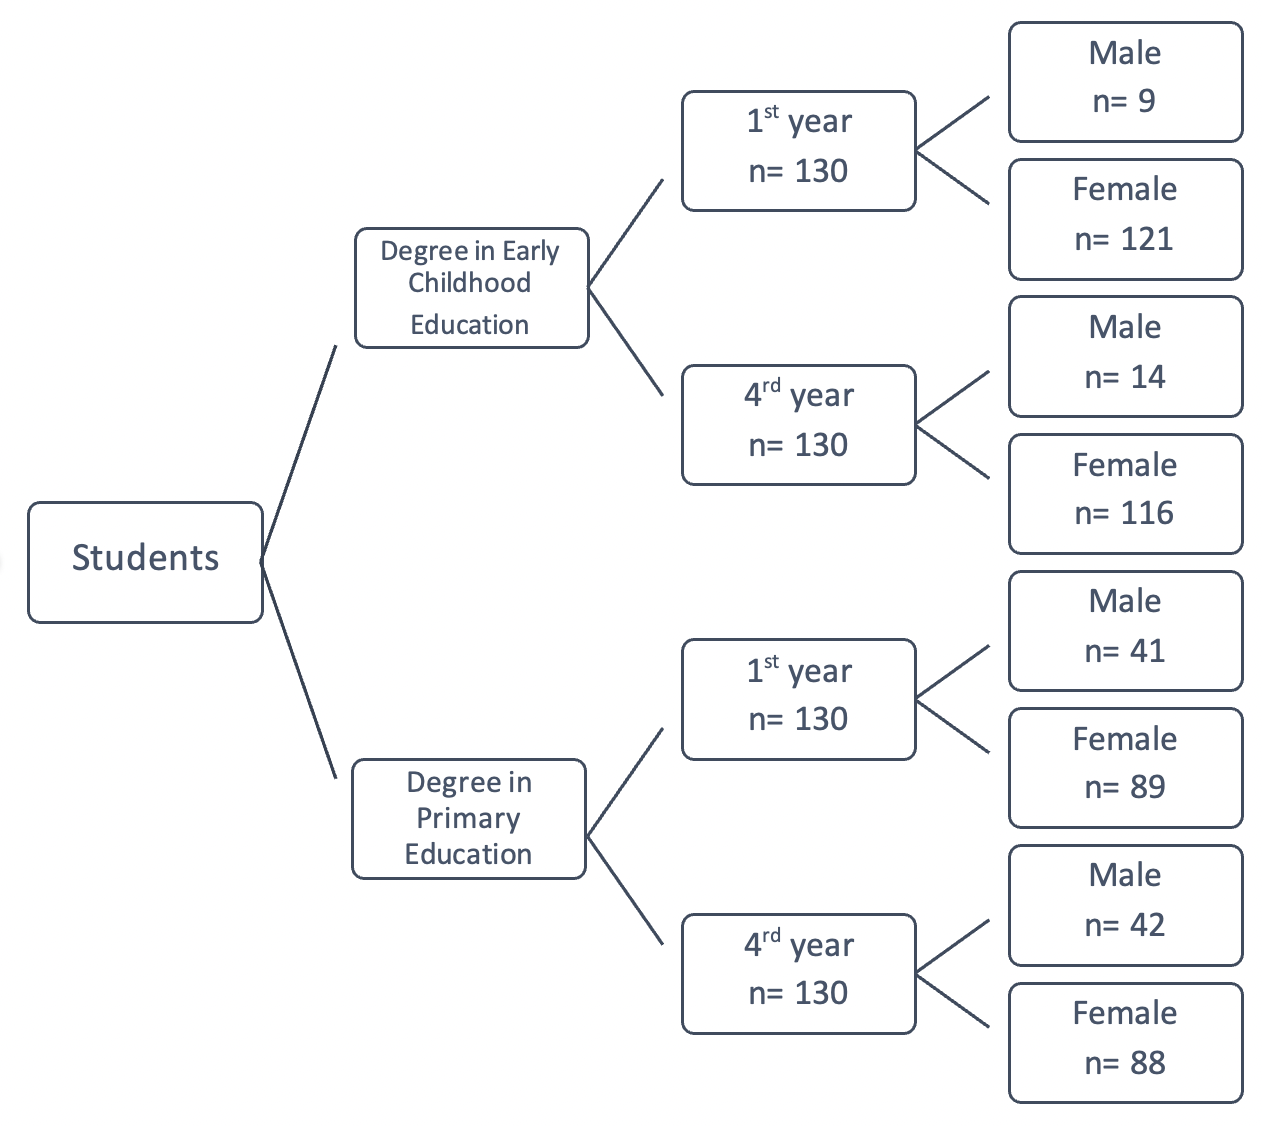
\includegraphics[width=0.85\textwidth]{Fig1.png}
 \caption{Distribution of the sample.}
 \label{fig01}
 \source{Own elaboration.}
\end{figure}

\subsection{Research instruments}\label{sec-fmt-manuscrito}
Two instruments were used to collect the data for this study. Before applying them, the participants were asked to sign an informed consent. First, a sociological questionnaire was passed with sociodemographic questions: age, sex, mother tongue, etc. Questions related to training were included: year and degree; and knowledge of foreign languages: language level according to the Common European Framework of Reference for Languages \cite{consejo_de_europa_marco_2002}, reading in foreign languages, etc. Second, an associative test was applied in Spanish, English and French. 

The use of this type of test is classic in studies of available lexicon and is based on the system of open lists with a duration of two minutes. Although the test included five centres of interest, in this work we are going to focus on the repertoires generated from “Reading”. In future research we will pay attention to the lexicon generated in the remaining four: “Teachers”, “Education”, “School: furniture and materials” and “Computers and the Internet”.

\subsection{Procedure}\label{sec-formato}
First, the sociological questionnaire was applied. Next, for the available lexicon test, 15 blank sheets of paper were given to the informants where they could write the words associated with each centre of interest in the three languages. In this way, lexical evocation processes were not interfered with \cite{santos_diaz_activacion_2020,santos_diaz_concepto_2022}. The research team projected the names of the centres of interest on the electronic board. The students copied them and evoked the related lexicon for 2 minutes, following the guidelines of the lexical availability studies \cite{lopez_gonzalez_disponibilidad_2014}. The tests were conducted first in Spanish, then in English, and finally in French. Students were instructed not to pay special attention to spell checking. This eliminated barriers to the detriment of lexical productivity, especially in the foreign language.

Once the questionnaire and the associative test were applied to the informants, an \textit{ad hoc} matrix was created where the different study variables were coded. This allowed a statistical approach to the data using the statistical package IBM SPSS v. 24.

For the edition of the lexical repertoires in Spanish, the guidelines of \textcite{samper-padilla_proyecto_2003} were followed. For the repertoires in French and English, those established by \textcite{de_la_maya_retamar_desarrollo_2015,mackey_vocabulaire_1971,santos_diaz_activacion_2020} were followed. However, in this work a broad lemmatization criterion has been followed and all the words evoked by the informants in each centre of interest have been admitted. This has made possible to better understand the relationships between words that occur and even explore newly created words.

After the lemmatization phase, the words separated by commas were organized around each informant coded according to the variables in a file (.txt) for each centre of interest and language. From this, the data was processed with the Dispogen II package \cite{echeverria_dispogen_2005}. The use of this package allowed, on the one hand, to obtain the available lexicon by applying the formula of \textcite{lopez-chavez_otro_1978} and, on the other hand, to generate associative graphs with DispoGrafo \cite{echeverria_dispografo:_2008}. In addition, to show a global vision of the most frequent words in each language, word clouds were configured with the Word Cloud Generator application, available on the web: \url{https://www.nubedepalabras.es/}.

The use of DispoGrafo made possible to analyse and measure the frequency of the set of words that make up the semantic network of a centre of interest \cite{collins_retrieval_1969,steyvers_large-scale_2005}. The name of the program itself provides relevant information about its objectives. “Dispo” refers to the methodology of lexical availability. “Graph” refers to the form acquired by the semantic networks resulting from the frequency calculation of the sequence of words. To generate the graphs \textcite{echeverria_dispografo:_2008} are based on the Graph Theory of the mathematical field. Each graph is composed of nodes that correspond to the words. These nodes join each other with edges depending on the relationships established between the words. The frequency of appearance of the same sequence or relationship as “book-library” will be determined by the weight of the edge.


\section{Results}\label{sec-modelo}

\subsection{General data according to language}
The informants have written a total of 13,380 words in the tests in the three languages. However, as \Cref{tab01} shows, the results have been very different depending on the language. Spanish is the language that registers the highest number of total words and presents an average of 14.56 words per informant. This is followed by English, which is usually the first foreign language, with 9.01 words per informant, and finally French, which corresponds in most cases to the second foreign language with 4.33 words per informant.

The cohesion index, calculated by dividing the mean number of words by the number of informants \cite{mena_disponibilidad_1986}, shows that the language with the greatest homogeneity is French, since it is the one that approaches 1. English and, finally, Spanish. This is because the level in French was lower than in the other languages and the lexical repertoire is less rich than in the other two languages (\Cref{tab01}).

\begin{table}[h!]
\centering
\begin{threeparttable}
\caption{Number of words and terms according to language.}
\label{tab01}
\begin{tabular}{l r r r r}
\toprule
 & Total Words & Average words & Total Terms & Cohesion index  \\
 \midrule
Spanish & 7,569 & 14.56 & 1,404 & 0.010   \\
English & 4,612 & 9.01 & 737 & 0.012  \\
French & 1,199 & 4.33 & 307 & 0.014 \\
\bottomrule
\end{tabular}
\source{Own elaboration.}
\end{threeparttable}
\end{table}

From a qualitative perspective, we are going to analyse the production of the first 20 most available words (see \Cref{apx-longtable}). The following similarities are observed in the three languages:

\begin{itemize}
    \item \textit{Libro, book, livre}. In all three languages it is the most available word.
    \item Leer, read, lire. The action of reading is the second most available word in a foreign language and in Spanish it ranks 10th.
    \item \textit{Biblioteca, library, bibliothèque}. It is the third most available word in all three languages.
    \item \textit{Novela, novel, roman}. It is the literary genre present in all three languages.
    \item \textit{Letra, letter, lettre}. In French and English, they are polysemous words that can mean letter. In Spanish and English, the term \textit{palabra}, \textit{word} also appears.
    \item \textit{Aprendizaje, learn, apprendre}. In Spanish the noun is used and in English and French the verb, but the relationship between reading and learning is observed.
    \item \textit{Cultura, culture, culture}. In all three languages, reading is associated with a cultural activity.
\end{itemize}

Regarding the similarities of Spanish in only one of the languages, the following words appear with English: 1) \textit{revista, magazine}; 2) \textit{periódico, newspaper}; 3) \textit{historia, history}; 4) \textit{imaginación, imagination}, and 5) \textit{aventura, adventure}. With French the coincidences are minor: 1) \textit{literatura, littérature [litterature]}, and 2) \textit{autor, auteur [author]}.

In both foreign languages the following words are repeated: 1) \textit{page} (English), \textit{page} (French). It is written the same in both languages; 2) \textit{education, éducation}; 3) \textit{write, écrire}. In addition, in English the noun that refers to the person is mentioned: \textit{writer} and 4) \textit{love}, \textit{amour}, reference is made to love, perhaps as a sign of love for reading.

Regarding words that only appear in the top 20 in a language, the following are recorded:

\begin{itemize}
    \item Spanish: \textit{cuento, conocimiento, diversión, lector} [\textit{story, knowledge, fun, reader}].
    \item English: \textit{paper}, and \textit{e-book}.
    \item French: \textit{compréhension, lecture, professeur, école, famille} [\textit{comprehension, reading, teacher, school,} and \textit{family}]. Perhaps due to lack of vocabulary, students have written the name of the centre of interest on more occasions: \textit{lecture} (21 informants, 7.21\% of the total). In addition, the allusion to education (\textit{professeur} and \textit{école}) [\textit{teacher} and \textit{school}] and \textit{famille} [family] continues, perhaps because they are the environments where reading is practiced and, also, because they are words related to the environment that are learned at basic user levels. according to the Common European Framework of Reference for Languages \cite{consejo_de_europa_marco_2002}. However, the types of reading are present in all three languages, although they are less available.
\end{itemize}

\Cref{fig2}, \Cref{fig3} and \Cref{fig4} show an overview of the lexicon available in the three languages in which the size of the words is conditioned by their frequency of appearance. In addition to the words mentioned above, they appear \textit{leer, relajación, revista, and periódico} [\textit{reading, relax, magazine,} and \textit{newspaper}]. In Spanish, the words that stand out the most are:\textit{ libro, cuento, biblioteca, and poesía} [\textit{book, story, library,} and \textit{poetry}]. On the other hand, in English the words attract attention: \textit{funny, story, children,} and \textit{fantasy}. In French, there are fewer words because far fewer terms have been recorded. In addition to those mentioned above, the following stand out: \textit{cahier, Le Petit prince, and culture} [\textit{notebook, The Little Prince} and \textit{culture}].

\begin{figure}[htbp]
 \centering
 \begin{minipage}{.30\textwidth}
 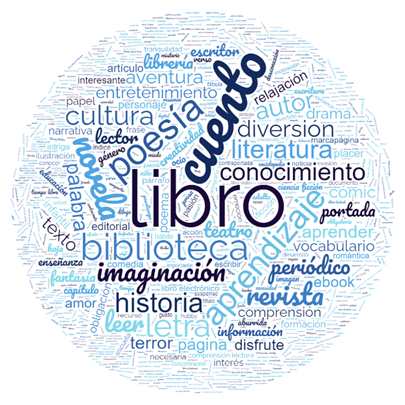
\includegraphics[width=\textwidth]{Fig2.png}
 \caption{Clouds of words of the available lexicon on reading by language - Spanish.}
 \label{fig2}
 \source{Own elaboration.}
 \end{minipage}%
 \qquad
 \begin{minipage}{0.30\textwidth}
 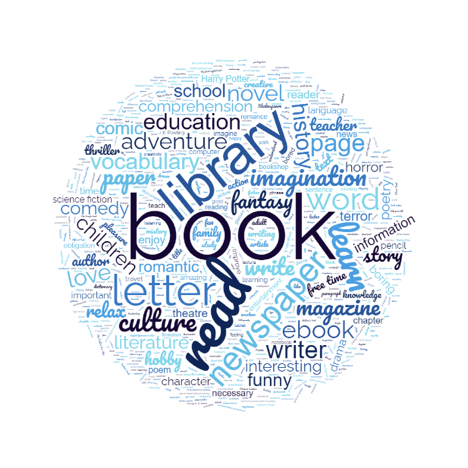
\includegraphics[width=\textwidth]{Fig3.png}
 \caption{Clouds of words of the available lexicon on reading by language - English.}
 \label{fig3}
 \source{Own elaboration.} 
 \end{minipage}%
  \qquad
 \begin{minipage}{0.30\textwidth}
 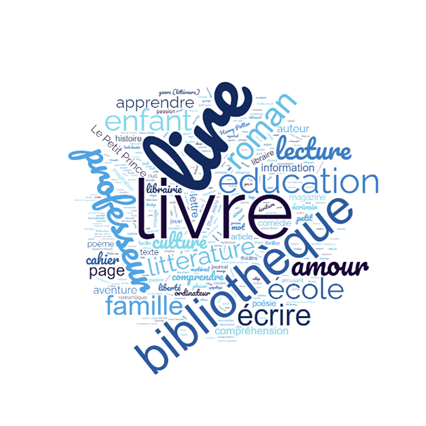
\includegraphics[width=\textwidth]{Fig4.png}
 \caption{Clouds of words of the available lexicon on reading by language - French.}
 \label{fig4}
 \source{Own elaboration.} 
 \end{minipage}%
\end{figure}

 To measure the statistical relationship between two continuous variables, such as the words in each of the languages, the Pearson correlation coefficient has been calculated. \Cref{tab02} shows that there is a positive bivariate correlation between the three possible pairs of combinations of the lists (Spanish-English, Spanish-French and English-French). This explains why informants who write more words in one language tend to write more in the other. In all cases, the correlation is significant at the 0.01 level, but the Pearson coefficient is higher when it comes to the Spanish-English relationship (0.558), while the rest of the correlations are very similar. Pearson’s correlation coefficient between English-French (0.185) and Spanish-French (0.189).

 \begin{table}[h!]
\begin{threeparttable}
\caption{Bivariate correlation between words according to language.}
\label{tab02}
\centering
\begin{tabular}{l l *{3}{S}}
\toprule
 & & {Words in Spanish} & {Words in English} & {Words in French} \\
\midrule
\multirow{3}{*}{Words in Spanish} & Pearson’s correlation & 1 & .558\tnote{**} & .189\tnote{**} \\
 & Sig. (bilateral) & & .000 & .000  \\
 & N & 520 & 520 & 520 \\
\multirow{3}{*}{Words in English} & Pearson’s correlation & .558\tnote{**} & 1 & .185\tnote{**} \\
 & Sig. (bilateral) & .000 & & .000 \\
 & N & 520 & 520 & 520 \\
\multirow{3}{*}{Words in French} & Pearson’s correlation & .189\tnote{**} & .185\tnote{**} & 1 \\
 & Sig. (bilateral) & .000 & .000 & \\
 & N & 520 & 520 & 520 \\
\bottomrule
\end{tabular}
\begin{tablenotes}
\item[**] The correlation is significant at the 0.01 level (2 tails).
\end{tablenotes}
\source{Own elaboration.}
\end{threeparttable}
\end{table}

 \subsection{From paper to digital reading: book versus e-book}\label{sec-organizacao}

The most available word in all three languages refers to the book. Although the format is not specified, in the three languages they are usually referred to differently when they want to refer to the electronic book, such as \textit{e-book}. In Spanish, \textit{libro electrónico [electronic book]} has been mentioned by 24 informants, which is equivalent to 4.2\% of the sample and \textit{libro digital [digital book]} by 12 informants (2.30\%). In English, digital book has been mentioned by 6 informants, 1.72\%, and electronic book by 4 (0.78\%). In French, livre digital [digital book] and \textit{livre électronique [electronic book]} have been mentioned by 1 informant (0.36\%).

\Cref{tab03} shows that in the three languages, most informants mentioned \textit{libro [book]}, \textit{book}, and \textit{livre [book]}. In English, that percentage rises to 92.77\%, followed by French, 78.70\%, and Spanish, 78.65\%. Nevertheless, when referring to the word \textit{e-book}, the percentage is much lower. In English it is more frequent, perhaps also because in Spanish we would have to add the synonyms used in the mother tongue (\textit{electronic book, digital book}). Thus, 10.16\% are registered in English, 8.65\% in Spanish and only 0.72\% in French.

\begin{table}[h!]
\centering
\begin{threeparttable}
\caption{Frequency and percentage of appearance of \textit{book} and \textit{e-book} in the three languages.}
\label{tab03}
\begin{tabular}{l l r r l r r}
\toprule
 & {Word} & {Frequency} & {\% Apparition} & {Word} & {Frequency} & {\% Apparition}   \\
 \midrule
Spanish & Libro & 409 & 78.653 & e-book & 45 & 8.654 \\
English & Book & 475 & 92.772 & e-book & 52 & 10.156 \\
French & Livre & 218 & 78.700 & e-book & 2 & 0.722 \\
\bottomrule
\end{tabular}
\source{Own elaboration.}
\end{threeparttable}
\end{table}

In addition to the word \textit{book}, there are other words that are usually more specific or simply integrate that root to give rise to other words. \Cref{tab04} shows the variants in the three languages. Thus, in Spanish 24 are registered, in English 11 and in French 4. In the three languages reference is made to the digital book and even in Spanish the difference between traditional book and paper book is marked.

\begin{table}[h!]
\centering
\begin{threeparttable}
\caption{Words derived from \textit{book}.}
\label{tab04}
\small
\begin{tabular}{p{6cm} p{3cm} p{3cm}}
\toprule
\textbf{Libro} & \textbf{Book} & \textbf{Livre} \\
\midrule
libro adulto, libro audiovisual, libro de aventura, libro de bolsillo, libro de ilustraciones, libro de imágenes, libro de mano, libro de papel, libro de película Disney, libro de terror, libro de texto, libro didáctico, \textbf{libro digital}, \textbf{libro electrónico}, libro en papel, \textbf{libro en tablet}, libro infantil, libro interactivo, libro interesante, libro olores, libro para niños, libro pedagógico, libro tecnológico, libro tradicional. & bookcase, book for children, bookmark, bookshelf, bookshop, \textbf{bookTube}, \textbf{book online}, \textbf{booktrailer}, \textbf{digital book}, notebook, workbook. & livre de l'élève, \textbf{livre digital}, \textbf{livre électronique}, livre maternelle.   \\
\bottomrule
\end{tabular}
\source{Own elaboration.}
\end{threeparttable}
\end{table}

Next, the most frequent associations will be shown in the three languages, both from \textit{book} and \textit{e-book}. The arrows indicate that the relationship occurs from the moment the informant mentioned the word \textit{book} to the next word. As for the number, it refers to the number of times that association is repeated.

From the term book, a subgraph has been generated with the DispoGrafo program (see \Cref{fig3}). Edges with a weight equal to or less than 3 have been eliminated, that is, those relationships between words that have only been produced by 3 informants. In addition, the nodes, that is, the sets of words, that had less than 2 connections have been eliminated. In this way, it is observed that there is no allusion to digital tools or new forms of reading on the Internet, since all the words belong to traditional genres (\textit{cuento, novela, poesía, comic}) [\textit{story, novel, poetry, comic}], they break down the unit of the \textit{libro} (\textit{texto, palabra, letra}) [\textit{text, word, letter}], refer to the type of reading (\textit{fantasía, aventura}) [\textit{fantasy, adventure}] and the main agents (\textit{autor, lector}) [\textit{author, reader}].

With respect to the subgraph created from \textit{e-book} (\Cref{fig5} and \Cref{fig6}), those relations with a weight equal to or greater than 2 have been maintained, since the word \textit{e-book} is less available and, therefore, the relations between words are less dense. The relationship is observed both with its synonym, \textit{libro electrónico} [\textit{electronic book}], and the contrast between \textit{libro} and \textit{papel} [\textit{book} and \textit{paper}]. In addition, \textit{tablet} and \textit{periódico} [\textit{newspaper}] support is included, and references are made to the \textit{grafía} [\textit{spelling}].

%Italicos

\begin{figure}[htbp]
 \centering
 \begin{minipage}{.45\textwidth}
 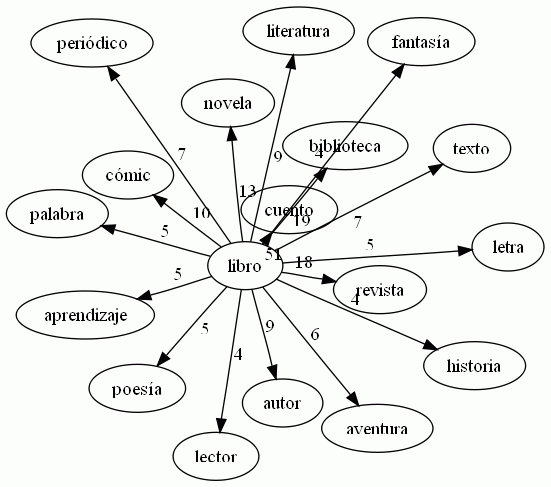
\includegraphics[width=\textwidth]{Fig5.png}
 \caption{Subgraph from \textit{libro} [\textit{book}].}
 \label{fig5}
 \source{Own elaboration.}
 \end{minipage}%
 \qquad
 \begin{minipage}{0.45\textwidth}
 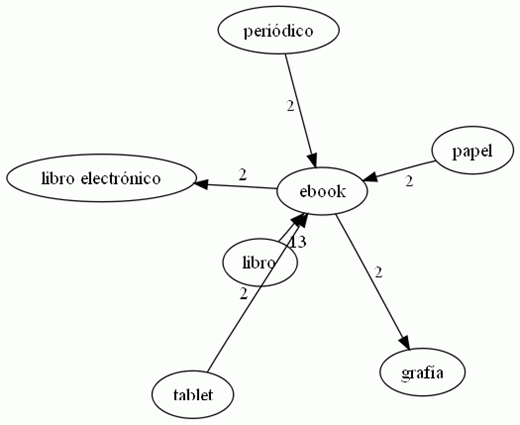
\includegraphics[width=\textwidth]{Fig6.png}
 \caption{Subgraph from \textit{e-book}.}
 \label{fig6}
 \source{Own elaboration.} 
 \end{minipage}%
\end{figure}

In \Cref{tab05}, the clusters or groups of words that are repeated in decreasing order have been included. The pair of words that is repeated the most is \textit{libro-cuento} [\textit{book-story}] (58 informants), followed by \textit{libro-biblioteca} [\textit{book-library}] (26), \textit{libro-leer} [\textit{book-reading}] (19) and \textit{libro-revista} [\textit{book-newspaper}] (19). The binomial \textit{libro-e-book} [\textit{book-e-book}] appears with 14 appearances and \textit{libro-tablet} [\textit{book-tablet}] with 8. Among the most common 3-word clusters, there is no allusion to digital tools. As for the clusters generated with e-book, it is related above all to virtual tools, such as its synonyms \textit{libro digital}, \textit{libro electrónico} [\textit{digital book}, \textit{electronic book}], as well as other supports such as tablets and analogous referents: \textit{libro, imprenta, papel} and \textit{físico} [\textit{book, press, paper} and \textit{physical}].

\begin{table}[h!]
\centering
\begin{threeparttable}
\caption{Clusters in Spanish.}
\label{tab05}
\centering
\begin{tabular}{l l l l}
\toprule
 \textbf{Quantity} & \textbf{Cluster} & \textbf{Quantity} & \textbf{Cluster} \\
 \midrule
58 & libro, cuento & 14 & libro, e-book \\
26 & libro, biblioteca & 3 & personaje, e-book \\
19 & libro, leer & 3 & periódico, e-book \\
19 & libro, revista & 3 & papel, e-book \\
14 & libro, e-book & 3 & revista, e-book \\
14 & libro, novela & 3 & escritor, e-book \\
14 & libro, autor & 2 & libro digital, e-book \\
13 & libro, literatura & 2 & e-book, libro electrónico \\
12 & libro, cómic & 2 & e-book, no obligación \\
12 & libro, página & 2 & e-book, imprenta \\
10 & libro, enciclopedia & 2 & e-book, grafía \\
8 & libro, lector & 2 & e-book, físico \\
8 & libro, texto & 2 & cuento, e-book \\
8 & libro, tablet & 2 & tablet, e-book \\
\bottomrule
\end{tabular}
\source{Own elaboration.}
\end{threeparttable}
\end{table}

In the subparagraphs in English, the relationships between words are weaker, so we have only eliminated relationship lower than 3 in \Cref{fig7} and lower that 1 in \Cref{fig8}. It is observed how \textit{book} is related to the educational field through \textit{school, teacher} and even \textit{learn} and \textit{vocabulary}. Also included are the verbs \textit{read} and \textit{write} and the nouns \textit{reader} and \textit{writer}. The only relationship with a digital tool is through \textit{e-book}.

Instead, in \Cref{fig8}, we see how \textit{e-book} is related to mail and what could perhaps refer to a \textit{tablet}. The informants have written \textit{table}, but this may be due to confusion with \textit{tablet}, since \textit{table} is not such a widely available word in the mother tongue.

\begin{figure}[htbp]
 \centering
 \begin{minipage}{.45\textwidth}
 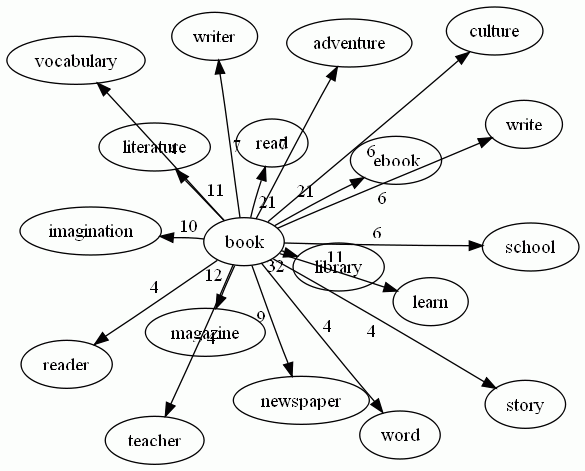
\includegraphics[width=\textwidth]{Fig7.png}
 \caption{Subgraph from book.}
 \label{fig7}
 \source{Own elaboration.}
 \end{minipage}%
 \qquad
 \begin{minipage}{0.45\textwidth}
 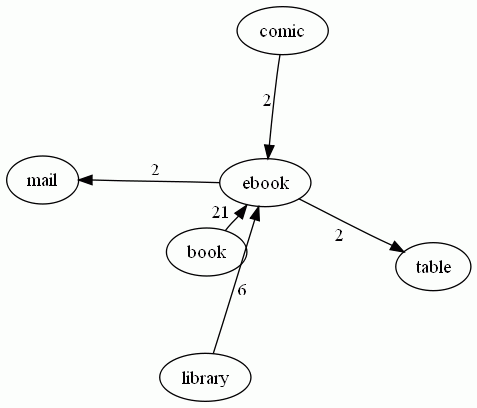
\includegraphics[width=\textwidth]{Fig8.png}
 \caption{Subgraph from e-book.}
 \label{fig8}
 \source{Own elaboration.} 
 \end{minipage}%
\end{figure}

Regarding the most frequent clusters (\Cref{tab06}), \textit{book} is associated with \textit{reading} (46) and with \textit{library} (41), unlike Spanish where the most frequent relationship was with \textit{cuento} [story]. As in Spanish, among the most frequent relationships of words, only \textit{e-book} is found as a digital tool. However, when the relationship between words and \textit{e-book} is analysed, \textit{tablet} and \textit{mail} do appear. As in paper books, \textit{library} also plays an essential role in the electronic format (11 records).

\begin{table}[h!]
\centering
\begin{threeparttable}
\caption{Clusters in English.}
\label{tab06}
\begin{tabular}{l l l l}
\toprule
 \textbf{Quantity} & \textbf{Cluster} & \textbf{Quantity} & \textbf{Cluster} \\
 \midrule
46 & book, read & 10 & Book, comic \\
41 & book, library & 4 & page, e-book \\
24 & book, e-book & 2 & history, e-book \\
23 & book, letter & 2 & letter, e-book \\
19 & newspaper, magazine & 2 & literature, e-book \\
17 & read, write & 2 & novel, e-book \\
14 & book, page & 2 & comic, e-book \\
14 & book, learn & 2 & e-book, Blue Jeans \\
13 & book, literature & 2 & e-book, table \\
12 & book, newspaper & 2 & e-book, mail \\
12 & book, magazine & 2 & newspaper, e-book \\
11 & book, novel & 2 & tablet, e-book \\
11 & book, imagination & 2 & paper, e-book \\
11 & library, e-book & 2 & funny, e-book \\
10 & book, write & 2 & culture, e-book \\
\bottomrule
\end{tabular}
\source{Own elaboration.}
\end{threeparttable}
\end{table}

In French relationships between words with a weight equal to or greater than 2 (\Cref{fig9}) or 1 (\Cref{fig10}) have been shown. There is no reference to digital tools with \textit{livre} [\textit{book}], perhaps because these words are usually anglicized, and the informants have preferred not to write them. As in English, \textit{livre} [\textit{book}] is limited to the school environment (\textit{école}) [\textit{school}] and the family (\textit{famille}). In the case of e-book, it has been related to the traditional format, \textit{livre} [\textit{book}], and to \textit{lecteur} [\textit{reader}], the adjective \textit{sympathique} [\textit{sympathetic}] and, perhaps, to the age at which it is most used, \textit{adulte} [\textit{adult}].

\begin{figure}[htbp]
 \centering
 \begin{minipage}{.45\textwidth}
 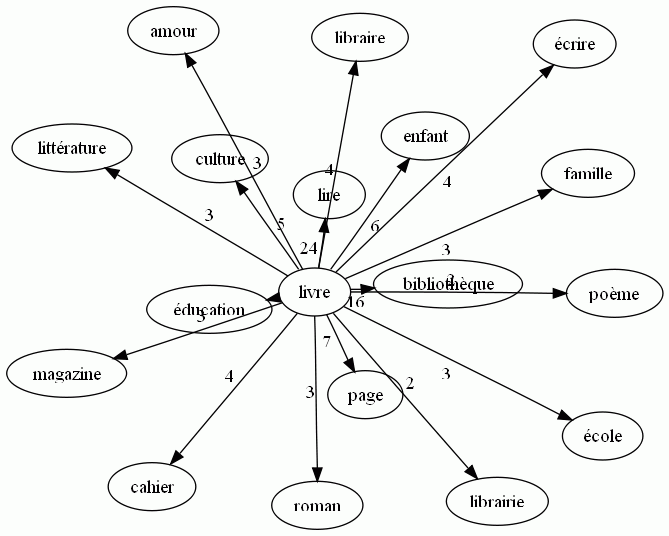
\includegraphics[width=\textwidth]{Fig9.png}
 \caption{Subgraph from \textit{livre} [\textit{book}].}
 \label{fig9}
 \source{Own elaboration.}
 \end{minipage}%
 \qquad
 \begin{minipage}{0.45\textwidth}
 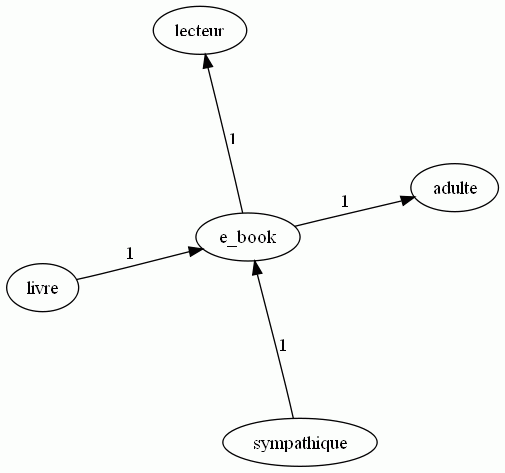
\includegraphics[width=\textwidth]{Fig10.png}
 \caption{Subgraph from e-\textit{book}.}
 \label{fig10}
 \source{Own elaboration.} 
 \end{minipage}%
\end{figure}

Because of the low appearance of \textit{e-book}, no cluster has been generated (\Cref{tab07}). With \textit{livre} [\textit{book}], the most common binomials are the same as in English (\textit{lire} and \textit{bibliothèque}) [\textit{reading} and \textit{library}]. In addition to the word relationships discussed above, \textit{amour} [\textit{love}] and the repetition of the \textit{reading} centre of interest stand out.

\begin{table}[h!]
\centering
\begin{threeparttable}
\caption{Clusters in French.}
\label{tab07}
\begin{tabular}{l l l l}
\toprule
 \textbf{Quantity} & \textbf{Cluster} & \textbf{Quantity} & \textbf{Cluster} \\
 \midrule
34 & livre, lire & 7 & lire, apprendre \\
18 & livre, bibliothèque & 5 & livre, amour \\
9 & livre, éducation & 5 & livre, article \\
9 & livre, enfant & 5 & livre, cahier \\
7 & livre, littérature & 5 & livre, famille \\
7 & livre, lecture & 5 & livre, culture \\
7 & livre, page & 5 & lire, écrire \\
7 & lire, lectura & & \\
\bottomrule
\end{tabular}
\source{Own elaboration.}
\end{threeparttable}
\end{table}

\subsection{New literary tools and practices}\label{sec-organizacao}
Despite the impact of new technologies \cite{alcocer_vazquez_practicas_2021,diaz_diaz_lectura_2022a,diaz-diaz_lector_2022b} in Spanish and French there is no word that refers to online literary practices or tools and virtual environments in promoting reading among the top twenty most available words. In English only appears \textit{e-book}.

\Cref{tab08} collects the entries that refer directly or indirectly to new literary practices or digital tools according to language. In addition to the \textit{e-book}, synonyms such as \textit{libro digital} and \textit{libro electrónico} [\textit{digital book} and \textit{electronic book}] appear. In English, self-created words such as \textit{book online} or \textit{technology book} appear. Regarding the type of support, there is \textit{Kindle}, \textit{tablet, iPad, iPod, televisión, teléfono, ordenador}, and \textit{pantalla} [\textit{Kindle, tablet, iPad, iPod, television, telephone, computer,} and \textit{screen}]. \textit{Internet} and \textit{technology} are mentioned in all three languages. In addition to the common word \textit{correo electrónico} [\textit{electronic mail}], \textit{Gmail} and \textit{Hotmail} appear.

Regarding the format, it has been collected: \textit{digital, formato digital} and \textit{soporte digital} [\textit{digital, digital format} and \textit{digital support}]. The informants have also mentioned \textit{formato físico, distinto formato} o \textit{soporte físico} [\textit{physical format, different format}, or \textit{physical support}]. In addition, with digital appears \textit{revista digital, periódico digital} and \textit{lectura digital} [\textit{digital review, digital newspaper}, and \textit{digital reading}]. In Spanish, three newspapers are mentioned after the entry of \textit{digital newspaper}, which are \textit{ABC, Marca,} and \textit{As}.

Along with this, the audiovisual medium is mentioned: \textit{cine, documental, película, película subtitulada, serie, subtítulo,} and \textit{versión original} [\textit{cinema, documentary, film, subtitled film, series, subtitle,} and \textit{original version}]. This is coupled with the verb \textit{ver} [\textit{to see}]. Also appear \textit{canción} [\textit{song}] and \textit{videojuego} [\textit{video game}].

\textit{Google} and \textit{Google Scholar} are registered as search engines. In addition, the \textit{YouTube} platform, and its specific use as a \textit{booktube}. Other formats used are the \textit{web page}, the \textit{blog}, and the \textit{vlog}.

\begin{small}
\renewcommand{\arraystretch}{1.5}
\begin{longtable}{
*{4}{l}
    % >{\raggedright\arraybackslash}p{0.3\textwidth}
    % p{0.3\textwidth}
    % p{0.2\textwidth}
    % p{0.2\textwidth}
    }
\caption{Lexicon related to the new literary practices.}
\label{tab08}
\\
\toprule
Category & Spanish & English & French \\
\midrule
\multirow{3}{*}{\textbf{Book tipes}} & e-book & e-book & e-book \\
& Libro digital & digital book & livre digital \\
& Libro electrónico & electronic book & livre électronique \\
\multirow{3}{*}{\textbf{Electronic reading tools}} & Kindle & Kindle & \\
& tablet & tablet & tablet \\
& & iPad & \\
& & iPod& \\
\multirow{3}{*}{\textbf{Platforms and the Internet}} & Correo electrónico & Email & \\
& Gmail & & \\
& & hotmail & \\
& Página web & & \\
& & bookTube & \\
& Youtube & & \\
& Blog & blog & blog \\
& & vlog & \\
& redes sociales & Social media & \\
& Google, Google académico & & \\
& Internet & internet & internet \\
& marcador & & \\
\textbf{Formats} & digital & digital & \\
& formato digital & & \\
& Revista digital & & \\
& Periódico digital & digital newspaper & \\
& Lectura digital & & \\
& PDF & & \\
& Word & & \\
& EPUB & & \\
\textbf{Audiovisual media} & Documental & & \\
& Cine & & cinéma \\
& Cinematográfica & & \\
& Película & film & \\
& Película subtitulada & & \\
& subtitle & & \\
& serie & soap opera & \\
& Versión original & & \\
& visualización & & \\
& & book trailer & \\
\textbf{Supports and tools} & soporte & support & \\
& Soporte digital & & \\
& Soporte físico & & \\
& Móvil  & Telephone & \\
& Televisión & Television & télévision \\
& & IT & \\
& ver & watch & \\
& tecnología & technology & \\
& ordenador & computer & ordinateur \\
& pantalla & screen & \\
& canción & song & \\
& & Videogame & \\
& vídeo & & vidéo \\
\bottomrule
\source{Own elaboration.}
\end{longtable}
\end{small}

\section{Discussion and conclusions}\label{sec-organizacao-latex}
The general objective of this research was to discover the concept of reading shared by future teachers of Early Childhood and Primary Education at the University of Malaga in Spanish, French and English. Special attention has been paid to the digital aspect. For this, the methodology of the available lexicon studies has been used \cite{lopez_gonzalez_disponibilidad_2014}. It has been found that this methodology is valid for making an adequate approach to the conceptions of teachers in training to detect opportunities to improve their instruction process.

From a quantitative perspective, the average number of words in Spanish per informant was 14.56. These results are lower than those obtained in previous research such as that of \textcite{herranz_llacer_palabra_2020,santos_diaz_activacion_2020}. However, they coincide with the findings of \textcite{santos_diaz_concepto_2022}. As for the foreign language, the average number of words per informant in English was 9.01, an issue that exceeds the results of the works by \textcite{de_la_maya_retamar_disponibilidad_2020,de_la_maya_retamar_habitos_2021,santos_diaz_concepto_2022}. In French, the average number of words per informant is 4.33, which offers better results than those of \textcite{santos_diaz_concepto_2022}.

From a qualitative perspective, the first thing that stands out is the fact that, even though the training plans include aspects related to the information society and include elements on multimodal and multimedia reading \cite{soto-vazquez_didactica_2022}, it seems that future teachers do not include these elements when referring to reading.

Specific objective 1 has focused on analysing the similarities and differences between the most available words in the three languages of the study. In this sense, it has been found that among the two most available words there are seven that are repeated in the three languages (book, library, novel, learning, letter, reading and culture), which corresponds to 35\%. From this it follows that reading is still understood in the traditional sense and, perhaps, it is difficult for future teachers to relate reading to book trailers, booktubers and other ways of promoting reading other than books \cite{alcocer_vazquez_practicas_2021,gomez_domingo_percepciones_2022}. These results coincide with those of the study by \textcite{castillo_fadic_lexico_2020}, carried out in Chile.

Specific objective 2 aimed to investigate the relationships between words that occur between the book (par excellence on paper) and the e-book in the three languages of the study. In accordance with this, it has been found that the relational lexicon is quite homogeneous in both languages and that there are hardly any words that lead us to think about the development of training for mediators within a multimodal society. These results coincide with those of \textcite{castillo_fadic_lexico_2020} and those of \textcite{juarez_calvillo_influencia_2019}.

Specific objective 3 sought to analyse the presence of digital tools and literary practices on the Internet through the concept of reading in the three languages of the study. In this regard, it has been found that, despite the frequent use of digital tools by young people \cite{rowsell_social_2018}, the words listed are few. These results contradict what was expressed by \textcite{cordon_garcia_socializacion_2023}, who reveal a new model of author and reader that takes social networks and fandom as a reference.

In reference to the limitations, we consider the results of this work should be understood as an attempt to understand what happened at the University of Malaga. However, we believe that the study should be extended to other universities. In the first instance, Andalusians and, in the second, from the rest of Spain.

Together with the above, just as \textcite{de_la_maya_retamar_disponibilidad_2020} pointed out in the Extremadura context, we consider that the limited lexicon available to our students in relation to multimodal and multimodal reading should be considered as an opportunity to open a reflective space about the training our students receive. As has been verified, it is necessary to make substantial improvements in the programming of degrees in education. This would help to connect the University with social advancement because, at times, it seems that this institution is not as up to date as it should be.

As a prospective line, it would be necessary to undertake a study to identify technicalities such as the one carried out by \textcite{santos_diaz_activacion_2020} to assess whether students can recognize the lexicon referring to new ways of reading \cite{amiama-espaillat_lectura_2017,cordon_garcia_socializacion_2023,diaz_diaz_lectura_2022a,diaz-diaz_lector_2022b}. In this way it will be possible to know if the informants have the passive knowledge of the vocabulary, but not the active one. Based on these results, more accurate solutions can be traced for the gradual improvement of teacher training, an objective that must be pursued by all nations.

\section{Funding}
This study arises from the collaboration between two research projects. One the one hand, the I D i project PID2021-126392OB-100 “Lecturas no ficcionales para la integración de ciudadanas y ciudadanos críticos en el nuevo ecosistema cultural” [Non-fictional readings for the integration of critical citizens in the new cultural ecosystem] that covers the study of reading. On the other hand, the I D I project “Observación del Pulso Social en Andalucía a través del análisis léxico (PULSO Andaluz)” [Observation of the Social Pulse in Andalusia through lexical analysis] (Ref. UMA20-FEDERJA-013) 

\printbibliography\label{sec-bib}
% if the text is not in Portuguese, it might be necessary to use the code below instead to print the correct ABNT abbreviations [s.n.], [s.l.]
%\begin{portuguese}
%\printbibliography[title={Bibliography}]
%\end{portuguese}


%full list: conceptualization,datacuration,formalanalysis,funding,investigation,methodology,projadm,resources,software,supervision,validation,visualization,writing,review
\begin{contributors}[sec-contributors]
\authorcontribution{Ester Trigo Ibáñez}[conceptualization,methodology,datacuration,formalanalysis,writing,review]
\authorcontribution{Inmaculada Clotilde Santos Díaz}[conceptualization,methodology,datacuration,formalanalysis,writing,review]
\end{contributors}


\newpage
\appendix 
\section{Appendix}\label{apx-longtable}
%20 More available words per language

\begin{small}
\renewcommand{\arraystretch}{1.5}
\begin{longtable}{
    % >{\raggedright\arraybackslash}p{0.1\textwidth}
    % p{0.2\textwidth}
    % p{0.2\textwidth}
    % p{0.1\textwidth}
    % p{0.2\textwidth}
    % p{0.2\textwidth}
    ll *{4}{S}
    }
\captionsetup{labelformat=empty}
%\captionsetup{labelformat=tablennumber}
\caption{20 More available words per language.}
%\caption*{20 More available words per language.}
%\label{anexo}
\\
\toprule
& {Term} & {Lexical availability index} & {Frequency} & {\% Apparition} & {Accumulated frequency} \\
\midrule
\multicolumn{6}{c}{More available words in Spanish} \\
\midrule
\textbf{1} & \textbf{Libro} & 0.70981 & 409 & 78.654 & 0.054 \\
2 & Cuento & 0.22854 & 168 & 32.308 & 0.076 \\
\textbf{3} & \textbf{Biblioteca} & 0.13913 & 111 & 21.346 & 0.091 \\
4 & Poesía & 0.12828 & 113 & 21.731 & 0.106 \\
\textbf{5} & \textbf{Novela} & 0.12695 & 105 & 20.192 & 0.120 \\
\textbf{6} & \textbf{Aprendizaje} & 0.12448 & 101 & 19.423 & 0.133 \\
\textbf{7} & \textbf{Letra} & 0.11319 & 95 & 18.269 & 0.146 \\
8 & Literatura & 0.10421 & 79 & 15.192 & 0.156 \\
9 & Imaginación & 0.10069 & 84 & 16.154 & 0.167 \\
\textbf{10} & \textbf{Leer} & 0.09863 & 73 & 14.038 & 0.177 \\
\textbf{11} & \textbf{Cultura} & 0.09811 & 82 & 15.769 & 0.188 \\
12 & Revista & 0.09770 & 82 & 15.769 & 0.198 \\
13 & Diversión & 0.08793 & 69 & 13.269 & 0.208 \\
14 & Historia & 0.08705 & 84 & 16.154 & 0.219 \\
15 & Autor & 0.08514 & 75 & 14.423 & 0.229 \\
16 & Periódico & 0.08200 & 68 & 13.077 & 0.238 \\
17 & Conocimiento & 0.07657 & 73 & 14.038 & 0.247 \\
18 & Lector & 0.07002 & 54 & 10.385 & 0.254 \\
19 & Palabra & 0.06962 & 63 & 12.115 & 0.263 \\
20 & Aventura & 0.06816 & 57 & 10.962 & 0.270 \\
\midrule
\multicolumn{6}{c}{More available words in English} \\
\midrule
& {Term} & {Lexical avalability index} & {Frequency} & {\% Apparition} & {Acumulated frequency} \\
\midrule
\textbf{1} & \textbf{Book} & 0.87228 & 475 & 92.773 & 0.103 \\
\textbf{2} & \textbf{Read} & 0.19009 & 122 & 23.828 & 0.129 \\
\textbf{3} & \textbf{Library} & 0.16002 & 115 & 22.461 & 0.154 \\
\textbf{4} & \textbf{Letter} & 0.12380 & 89 & 17.383 & 0.174 \\
\textbf{5} & \textbf{Learn} & 0.10234 & 74 & 14.453 & 0.190 \\
6 & Word & 0.09232 & 68 & 13.281 & 0.204 \\
7 & Newspaper & 0.09126 & 70 & 13.672 & 0.220 \\
\textbf{8} & \textbf{Culture} & 0.07701 & 59 & 11.523 & 0.232 \\
9 & E-book & 0.07255 & 52 & 10.156 & 0.244 \\
10 & Writer & 0.06942 & 53 & 10.352 & 0.255 \\
11 & Imagination & 0.06788 & 51 & 9.961 & 0.266 \\
12 & Page & 0.06737 & 51 & 9.961 & 0.277 \\
13 & Love & 0.06531 & 50 & 9.766 & 0.288 \\
14 & Write & 0.06467 & 50 & 9.766 & 0.299 \\
\textbf{15} & \textbf{Novel} & 0.06426 & 47 & 9.180 & 0.309 \\
16 & Education & 0.06353 & 50 & 9.766 & 0.320 \\
17 & Adventure & 0.06276 & 50 & 9.766 & 0.331 \\
18 & Magazine & 0.05957 & 49 & 9.570 & 0.342 \\
19 & Paper & 0.05905 & 46 & 8.984 & 0.351 \\
20 & History & 0.05785 & 48 & 9.375 & 0.362 \\
\midrule
\multicolumn{6}{c}{More available words in French} \\
\midrule
& {Term} & {Lexical avalability index} & {Frequency} & {\% Apparition} & {Acumulated frequency} \\
\midrule
\textbf{1} & \textbf{Livre} & 0.75086 & 218 & 78.700 & 0.182 \\
\textbf{2} & \textbf{Lire} & 0.21216 & 68 & 24.549 & 0.239 \\
\textbf{3} & \textbf{Bibliothèque} & 0.10936 & 40 & 14.440 & 0.272 \\
4 & Éducation & 0.07462 & 29 & 10.469 & 0.296 \\
5 & Professeur & 0.07184 & 28 & 10.108 & 0.319 \\
6 & Enfant & 0.07147 & 25 & 9.025 & 0.340 \\
7 & Écrire & 0.06537 & 24 & 8.664 & 0.360 \\
8 & École & 0.06422 & 24 & 8.664 & 0.380 \\
9 & Lecture & 0.06300 & 21 & 7.581 & 0.398 \\
\textbf{10} & \textbf{Roman} & 0.06187 & 27 & 9.747 & 0.420 \\
11 & Amour & 0.05839 & 25 & 9.025 & 0.441 \\
12 & Famille & 0.05233 & 21 & 7.581 & 0.459 \\
13 & Littérature & 0.04805 & 19 & 6.859 & 0.475 \\
\textbf{14} & \textbf{Culture} & 0.04472 & 16 & 5.776 & 0.488 \\
15 & Page & 0.03754 & 14 & 5.054 & 0.500 \\
16 & Cahier & 0.03635 & 11 & 3.971 & 0.509 \\
\textbf{17} & \textbf{Apprendre} & 0.02893 & 13 & 4.693 & 0.520 \\
\textbf{18} & \textbf{Lettre} & 0.02544 & 9 & 3.249 & 0.527 \\
19 & Auteur & 0.02521 & 9 & 3.249 & 0.535 \\
20 & Compréhension & 0.02364 & 8 & 2.888 & 0.541 \\
\bottomrule
\source{Own elaboration.}
\end{longtable}
\end{small}


\end{document}

